\documentclass{article} % For LaTeX2e
\usepackage{iclr2026_conference,times}
%%%%% NEW MATH DEFINITIONS %%%%%

\usepackage{amsmath,amsfonts,bm}

% Mark sections of captions for referring to divisions of figures
\newcommand{\figleft}{{\em (Left)}}
\newcommand{\figcenter}{{\em (Center)}}
\newcommand{\figright}{{\em (Right)}}
\newcommand{\figtop}{{\em (Top)}}
\newcommand{\figbottom}{{\em (Bottom)}}
\newcommand{\captiona}{{\em (a)}}
\newcommand{\captionb}{{\em (b)}}
\newcommand{\captionc}{{\em (c)}}
\newcommand{\captiond}{{\em (d)}}

% Highlight a newly defined term
\newcommand{\newterm}[1]{{\bf #1}}


% Figure reference, lower-case.
\def\figref#1{figure~\ref{#1}}
% Figure reference, capital. For start of sentence
\def\Figref#1{Figure~\ref{#1}}
\def\twofigref#1#2{figures \ref{#1} and \ref{#2}}
\def\quadfigref#1#2#3#4{figures \ref{#1}, \ref{#2}, \ref{#3} and \ref{#4}}
% Section reference, lower-case.
\def\secref#1{section~\ref{#1}}
% Section reference, capital.
\def\Secref#1{Section~\ref{#1}}
% Reference to two sections.
\def\twosecrefs#1#2{sections \ref{#1} and \ref{#2}}
% Reference to three sections.
\def\secrefs#1#2#3{sections \ref{#1}, \ref{#2} and \ref{#3}}
% Reference to an equation, lower-case.
\def\eqref#1{equation~\ref{#1}}
% Reference to an equation, upper case
\def\Eqref#1{Equation~\ref{#1}}
% A raw reference to an equation---avoid using if possible
\def\plaineqref#1{\ref{#1}}
% Reference to a chapter, lower-case.
\def\chapref#1{chapter~\ref{#1}}
% Reference to an equation, upper case.
\def\Chapref#1{Chapter~\ref{#1}}
% Reference to a range of chapters
\def\rangechapref#1#2{chapters\ref{#1}--\ref{#2}}
% Reference to an algorithm, lower-case.
\def\algref#1{algorithm~\ref{#1}}
% Reference to an algorithm, upper case.
\def\Algref#1{Algorithm~\ref{#1}}
\def\twoalgref#1#2{algorithms \ref{#1} and \ref{#2}}
\def\Twoalgref#1#2{Algorithms \ref{#1} and \ref{#2}}
% Reference to a part, lower case
\def\partref#1{part~\ref{#1}}
% Reference to a part, upper case
\def\Partref#1{Part~\ref{#1}}
\def\twopartref#1#2{parts \ref{#1} and \ref{#2}}

\def\ceil#1{\lceil #1 \rceil}
\def\floor#1{\lfloor #1 \rfloor}
\def\1{\bm{1}}
\newcommand{\train}{\mathcal{D}}
\newcommand{\valid}{\mathcal{D_{\mathrm{valid}}}}
\newcommand{\test}{\mathcal{D_{\mathrm{test}}}}

\def\eps{{\epsilon}}


% Random variables
\def\reta{{\textnormal{$\eta$}}}
\def\ra{{\textnormal{a}}}
\def\rb{{\textnormal{b}}}
\def\rc{{\textnormal{c}}}
\def\rd{{\textnormal{d}}}
\def\re{{\textnormal{e}}}
\def\rf{{\textnormal{f}}}
\def\rg{{\textnormal{g}}}
\def\rh{{\textnormal{h}}}
\def\ri{{\textnormal{i}}}
\def\rj{{\textnormal{j}}}
\def\rk{{\textnormal{k}}}
\def\rl{{\textnormal{l}}}
% rm is already a command, just don't name any random variables m
\def\rn{{\textnormal{n}}}
\def\ro{{\textnormal{o}}}
\def\rp{{\textnormal{p}}}
\def\rq{{\textnormal{q}}}
\def\rr{{\textnormal{r}}}
\def\rs{{\textnormal{s}}}
\def\rt{{\textnormal{t}}}
\def\ru{{\textnormal{u}}}
\def\rv{{\textnormal{v}}}
\def\rw{{\textnormal{w}}}
\def\rx{{\textnormal{x}}}
\def\ry{{\textnormal{y}}}
\def\rz{{\textnormal{z}}}

% Random vectors
\def\rvepsilon{{\mathbf{\epsilon}}}
\def\rvtheta{{\mathbf{\theta}}}
\def\rva{{\mathbf{a}}}
\def\rvb{{\mathbf{b}}}
\def\rvc{{\mathbf{c}}}
\def\rvd{{\mathbf{d}}}
\def\rve{{\mathbf{e}}}
\def\rvf{{\mathbf{f}}}
\def\rvg{{\mathbf{g}}}
\def\rvh{{\mathbf{h}}}
\def\rvu{{\mathbf{i}}}
\def\rvj{{\mathbf{j}}}
\def\rvk{{\mathbf{k}}}
\def\rvl{{\mathbf{l}}}
\def\rvm{{\mathbf{m}}}
\def\rvn{{\mathbf{n}}}
\def\rvo{{\mathbf{o}}}
\def\rvp{{\mathbf{p}}}
\def\rvq{{\mathbf{q}}}
\def\rvr{{\mathbf{r}}}
\def\rvs{{\mathbf{s}}}
\def\rvt{{\mathbf{t}}}
\def\rvu{{\mathbf{u}}}
\def\rvv{{\mathbf{v}}}
\def\rvw{{\mathbf{w}}}
\def\rvx{{\mathbf{x}}}
\def\rvy{{\mathbf{y}}}
\def\rvz{{\mathbf{z}}}

% Elements of random vectors
\def\erva{{\textnormal{a}}}
\def\ervb{{\textnormal{b}}}
\def\ervc{{\textnormal{c}}}
\def\ervd{{\textnormal{d}}}
\def\erve{{\textnormal{e}}}
\def\ervf{{\textnormal{f}}}
\def\ervg{{\textnormal{g}}}
\def\ervh{{\textnormal{h}}}
\def\ervi{{\textnormal{i}}}
\def\ervj{{\textnormal{j}}}
\def\ervk{{\textnormal{k}}}
\def\ervl{{\textnormal{l}}}
\def\ervm{{\textnormal{m}}}
\def\ervn{{\textnormal{n}}}
\def\ervo{{\textnormal{o}}}
\def\ervp{{\textnormal{p}}}
\def\ervq{{\textnormal{q}}}
\def\ervr{{\textnormal{r}}}
\def\ervs{{\textnormal{s}}}
\def\ervt{{\textnormal{t}}}
\def\ervu{{\textnormal{u}}}
\def\ervv{{\textnormal{v}}}
\def\ervw{{\textnormal{w}}}
\def\ervx{{\textnormal{x}}}
\def\ervy{{\textnormal{y}}}
\def\ervz{{\textnormal{z}}}

% Random matrices
\def\rmA{{\mathbf{A}}}
\def\rmB{{\mathbf{B}}}
\def\rmC{{\mathbf{C}}}
\def\rmD{{\mathbf{D}}}
\def\rmE{{\mathbf{E}}}
\def\rmF{{\mathbf{F}}}
\def\rmG{{\mathbf{G}}}
\def\rmH{{\mathbf{H}}}
\def\rmI{{\mathbf{I}}}
\def\rmJ{{\mathbf{J}}}
\def\rmK{{\mathbf{K}}}
\def\rmL{{\mathbf{L}}}
\def\rmM{{\mathbf{M}}}
\def\rmN{{\mathbf{N}}}
\def\rmO{{\mathbf{O}}}
\def\rmP{{\mathbf{P}}}
\def\rmQ{{\mathbf{Q}}}
\def\rmR{{\mathbf{R}}}
\def\rmS{{\mathbf{S}}}
\def\rmT{{\mathbf{T}}}
\def\rmU{{\mathbf{U}}}
\def\rmV{{\mathbf{V}}}
\def\rmW{{\mathbf{W}}}
\def\rmX{{\mathbf{X}}}
\def\rmY{{\mathbf{Y}}}
\def\rmZ{{\mathbf{Z}}}

% Elements of random matrices
\def\ermA{{\textnormal{A}}}
\def\ermB{{\textnormal{B}}}
\def\ermC{{\textnormal{C}}}
\def\ermD{{\textnormal{D}}}
\def\ermE{{\textnormal{E}}}
\def\ermF{{\textnormal{F}}}
\def\ermG{{\textnormal{G}}}
\def\ermH{{\textnormal{H}}}
\def\ermI{{\textnormal{I}}}
\def\ermJ{{\textnormal{J}}}
\def\ermK{{\textnormal{K}}}
\def\ermL{{\textnormal{L}}}
\def\ermM{{\textnormal{M}}}
\def\ermN{{\textnormal{N}}}
\def\ermO{{\textnormal{O}}}
\def\ermP{{\textnormal{P}}}
\def\ermQ{{\textnormal{Q}}}
\def\ermR{{\textnormal{R}}}
\def\ermS{{\textnormal{S}}}
\def\ermT{{\textnormal{T}}}
\def\ermU{{\textnormal{U}}}
\def\ermV{{\textnormal{V}}}
\def\ermW{{\textnormal{W}}}
\def\ermX{{\textnormal{X}}}
\def\ermY{{\textnormal{Y}}}
\def\ermZ{{\textnormal{Z}}}

% Vectors
\def\vzero{{\bm{0}}}
\def\vone{{\bm{1}}}
\def\vmu{{\bm{\mu}}}
\def\vtheta{{\bm{\theta}}}
\def\va{{\bm{a}}}
\def\vb{{\bm{b}}}
\def\vc{{\bm{c}}}
\def\vd{{\bm{d}}}
\def\ve{{\bm{e}}}
\def\vf{{\bm{f}}}
\def\vg{{\bm{g}}}
\def\vh{{\bm{h}}}
\def\vi{{\bm{i}}}
\def\vj{{\bm{j}}}
\def\vk{{\bm{k}}}
\def\vl{{\bm{l}}}
\def\vm{{\bm{m}}}
\def\vn{{\bm{n}}}
\def\vo{{\bm{o}}}
\def\vp{{\bm{p}}}
\def\vq{{\bm{q}}}
\def\vr{{\bm{r}}}
\def\vs{{\bm{s}}}
\def\vt{{\bm{t}}}
\def\vu{{\bm{u}}}
\def\vv{{\bm{v}}}
\def\vw{{\bm{w}}}
\def\vx{{\bm{x}}}
\def\vy{{\bm{y}}}
\def\vz{{\bm{z}}}

% Elements of vectors
\def\evalpha{{\alpha}}
\def\evbeta{{\beta}}
\def\evepsilon{{\epsilon}}
\def\evlambda{{\lambda}}
\def\evomega{{\omega}}
\def\evmu{{\mu}}
\def\evpsi{{\psi}}
\def\evsigma{{\sigma}}
\def\evtheta{{\theta}}
\def\eva{{a}}
\def\evb{{b}}
\def\evc{{c}}
\def\evd{{d}}
\def\eve{{e}}
\def\evf{{f}}
\def\evg{{g}}
\def\evh{{h}}
\def\evi{{i}}
\def\evj{{j}}
\def\evk{{k}}
\def\evl{{l}}
\def\evm{{m}}
\def\evn{{n}}
\def\evo{{o}}
\def\evp{{p}}
\def\evq{{q}}
\def\evr{{r}}
\def\evs{{s}}
\def\evt{{t}}
\def\evu{{u}}
\def\evv{{v}}
\def\evw{{w}}
\def\evx{{x}}
\def\evy{{y}}
\def\evz{{z}}

% Matrix
\def\mA{{\bm{A}}}
\def\mB{{\bm{B}}}
\def\mC{{\bm{C}}}
\def\mD{{\bm{D}}}
\def\mE{{\bm{E}}}
\def\mF{{\bm{F}}}
\def\mG{{\bm{G}}}
\def\mH{{\bm{H}}}
\def\mI{{\bm{I}}}
\def\mJ{{\bm{J}}}
\def\mK{{\bm{K}}}
\def\mL{{\bm{L}}}
\def\mM{{\bm{M}}}
\def\mN{{\bm{N}}}
\def\mO{{\bm{O}}}
\def\mP{{\bm{P}}}
\def\mQ{{\bm{Q}}}
\def\mR{{\bm{R}}}
\def\mS{{\bm{S}}}
\def\mT{{\bm{T}}}
\def\mU{{\bm{U}}}
\def\mV{{\bm{V}}}
\def\mW{{\bm{W}}}
\def\mX{{\bm{X}}}
\def\mY{{\bm{Y}}}
\def\mZ{{\bm{Z}}}
\def\mBeta{{\bm{\beta}}}
\def\mPhi{{\bm{\Phi}}}
\def\mLambda{{\bm{\Lambda}}}
\def\mSigma{{\bm{\Sigma}}}

% Tensor
\DeclareMathAlphabet{\mathsfit}{\encodingdefault}{\sfdefault}{m}{sl}
\SetMathAlphabet{\mathsfit}{bold}{\encodingdefault}{\sfdefault}{bx}{n}
\newcommand{\tens}[1]{\bm{\mathsfit{#1}}}
\def\tA{{\tens{A}}}
\def\tB{{\tens{B}}}
\def\tC{{\tens{C}}}
\def\tD{{\tens{D}}}
\def\tE{{\tens{E}}}
\def\tF{{\tens{F}}}
\def\tG{{\tens{G}}}
\def\tH{{\tens{H}}}
\def\tI{{\tens{I}}}
\def\tJ{{\tens{J}}}
\def\tK{{\tens{K}}}
\def\tL{{\tens{L}}}
\def\tM{{\tens{M}}}
\def\tN{{\tens{N}}}
\def\tO{{\tens{O}}}
\def\tP{{\tens{P}}}
\def\tQ{{\tens{Q}}}
\def\tR{{\tens{R}}}
\def\tS{{\tens{S}}}
\def\tT{{\tens{T}}}
\def\tU{{\tens{U}}}
\def\tV{{\tens{V}}}
\def\tW{{\tens{W}}}
\def\tX{{\tens{X}}}
\def\tY{{\tens{Y}}}
\def\tZ{{\tens{Z}}}


% Graph
\def\gA{{\mathcal{A}}}
\def\gB{{\mathcal{B}}}
\def\gC{{\mathcal{C}}}
\def\gD{{\mathcal{D}}}
\def\gE{{\mathcal{E}}}
\def\gF{{\mathcal{F}}}
\def\gG{{\mathcal{G}}}
\def\gH{{\mathcal{H}}}
\def\gI{{\mathcal{I}}}
\def\gJ{{\mathcal{J}}}
\def\gK{{\mathcal{K}}}
\def\gL{{\mathcal{L}}}
\def\gM{{\mathcal{M}}}
\def\gN{{\mathcal{N}}}
\def\gO{{\mathcal{O}}}
\def\gP{{\mathcal{P}}}
\def\gQ{{\mathcal{Q}}}
\def\gR{{\mathcal{R}}}
\def\gS{{\mathcal{S}}}
\def\gT{{\mathcal{T}}}
\def\gU{{\mathcal{U}}}
\def\gV{{\mathcal{V}}}
\def\gW{{\mathcal{W}}}
\def\gX{{\mathcal{X}}}
\def\gY{{\mathcal{Y}}}
\def\gZ{{\mathcal{Z}}}

% Sets
\def\sA{{\mathbb{A}}}
\def\sB{{\mathbb{B}}}
\def\sC{{\mathbb{C}}}
\def\sD{{\mathbb{D}}}
% Don't use a set called E, because this would be the same as our symbol
% for expectation.
\def\sF{{\mathbb{F}}}
\def\sG{{\mathbb{G}}}
\def\sH{{\mathbb{H}}}
\def\sI{{\mathbb{I}}}
\def\sJ{{\mathbb{J}}}
\def\sK{{\mathbb{K}}}
\def\sL{{\mathbb{L}}}
\def\sM{{\mathbb{M}}}
\def\sN{{\mathbb{N}}}
\def\sO{{\mathbb{O}}}
\def\sP{{\mathbb{P}}}
\def\sQ{{\mathbb{Q}}}
\def\sR{{\mathbb{R}}}
\def\sS{{\mathbb{S}}}
\def\sT{{\mathbb{T}}}
\def\sU{{\mathbb{U}}}
\def\sV{{\mathbb{V}}}
\def\sW{{\mathbb{W}}}
\def\sX{{\mathbb{X}}}
\def\sY{{\mathbb{Y}}}
\def\sZ{{\mathbb{Z}}}

% Entries of a matrix
\def\emLambda{{\Lambda}}
\def\emA{{A}}
\def\emB{{B}}
\def\emC{{C}}
\def\emD{{D}}
\def\emE{{E}}
\def\emF{{F}}
\def\emG{{G}}
\def\emH{{H}}
\def\emI{{I}}
\def\emJ{{J}}
\def\emK{{K}}
\def\emL{{L}}
\def\emM{{M}}
\def\emN{{N}}
\def\emO{{O}}
\def\emP{{P}}
\def\emQ{{Q}}
\def\emR{{R}}
\def\emS{{S}}
\def\emT{{T}}
\def\emU{{U}}
\def\emV{{V}}
\def\emW{{W}}
\def\emX{{X}}
\def\emY{{Y}}
\def\emZ{{Z}}
\def\emSigma{{\Sigma}}

% entries of a tensor
% Same font as tensor, without \bm wrapper
\newcommand{\etens}[1]{\mathsfit{#1}}
\def\etLambda{{\etens{\Lambda}}}
\def\etA{{\etens{A}}}
\def\etB{{\etens{B}}}
\def\etC{{\etens{C}}}
\def\etD{{\etens{D}}}
\def\etE{{\etens{E}}}
\def\etF{{\etens{F}}}
\def\etG{{\etens{G}}}
\def\etH{{\etens{H}}}
\def\etI{{\etens{I}}}
\def\etJ{{\etens{J}}}
\def\etK{{\etens{K}}}
\def\etL{{\etens{L}}}
\def\etM{{\etens{M}}}
\def\etN{{\etens{N}}}
\def\etO{{\etens{O}}}
\def\etP{{\etens{P}}}
\def\etQ{{\etens{Q}}}
\def\etR{{\etens{R}}}
\def\etS{{\etens{S}}}
\def\etT{{\etens{T}}}
\def\etU{{\etens{U}}}
\def\etV{{\etens{V}}}
\def\etW{{\etens{W}}}
\def\etX{{\etens{X}}}
\def\etY{{\etens{Y}}}
\def\etZ{{\etens{Z}}}

% The true underlying data generating distribution
\newcommand{\pdata}{p_{\rm{data}}}
% The empirical distribution defined by the training set
\newcommand{\ptrain}{\hat{p}_{\rm{data}}}
\newcommand{\Ptrain}{\hat{P}_{\rm{data}}}
% The model distribution
\newcommand{\pmodel}{p_{\rm{model}}}
\newcommand{\Pmodel}{P_{\rm{model}}}
\newcommand{\ptildemodel}{\tilde{p}_{\rm{model}}}
% Stochastic autoencoder distributions
\newcommand{\pencode}{p_{\rm{encoder}}}
\newcommand{\pdecode}{p_{\rm{decoder}}}
\newcommand{\precons}{p_{\rm{reconstruct}}}

\newcommand{\laplace}{\mathrm{Laplace}} % Laplace distribution

\newcommand{\E}{\mathbb{E}}
\newcommand{\Ls}{\mathcal{L}}
\newcommand{\R}{\mathbb{R}}
\newcommand{\emp}{\tilde{p}}
\newcommand{\lr}{\alpha}
\newcommand{\reg}{\lambda}
\newcommand{\rect}{\mathrm{rectifier}}
\newcommand{\softmax}{\mathrm{softmax}}
\newcommand{\sigmoid}{\sigma}
\newcommand{\softplus}{\zeta}
\newcommand{\KL}{D_{\mathrm{KL}}}
\newcommand{\Var}{\mathrm{Var}}
\newcommand{\standarderror}{\mathrm{SE}}
\newcommand{\Cov}{\mathrm{Cov}}
% Wolfram Mathworld says $L^2$ is for function spaces and $\ell^2$ is for vectors
% But then they seem to use $L^2$ for vectors throughout the site, and so does
% wikipedia.
\newcommand{\normlzero}{L^0}
\newcommand{\normlone}{L^1}
\newcommand{\normltwo}{L^2}
\newcommand{\normlp}{L^p}
\newcommand{\normmax}{L^\infty}

\newcommand{\parents}{Pa} % See usage in notation.tex. Chosen to match Daphne's book.

\DeclareMathOperator*{\argmax}{arg\,max}
\DeclareMathOperator*{\argmin}{arg\,min}

\DeclareMathOperator{\sign}{sign}
\DeclareMathOperator{\Tr}{Tr}
\let\ab\allowbreak

\usepackage{hyperref}
\usepackage{url}
\usepackage{booktabs}
\usepackage{graphicx}
\usepackage{xcolor}
\usepackage{enumitem}
\usepackage{amsmath}
\setlist{nosep,leftmargin=*}
\newcommand{\todo}[1]{\textcolor{red}{\textbf{[TODO: #1]}}}

\title{Does Talking Help a Squad of Language Models? \\ Communication, Memory and Post-Training in SMACv2}

\author{Ivy (Ning) Zhang \\
Stanford University \\
\texttt{para2046@stanford.edu}}

\iclrfinalcopy
\begin{document}
\maketitle

\section{Introduction}
Teams of LLM agents are increasingly asked to act together while each sees only part of the world.
We study the smallest such setting that still needs real-time coordination: a StarCraft~II squad in
which \emph{every unit is a separate copy of a language model} that reads a text description of what
its own unit sees and returns one order per step. We ask: (Q1) Does a communication channel between
the copies help, and does the answer depend on model size? (Q2) Does a short per-unit memory of one's
own recent actions and their outcomes help? (Q3) Can a small open model (Gemma~4 E4B) learn to play
from a larger one (Gemma~4 31B)? (Q4) Can multi-agent RL (MAPPO) against the game's AI improve
it further? (Q5) Where do the gains come from: which behaviours change? All conditions share one
system prompt that states only the game rules: it contains no tactics, so any coordination we observe
(e.g.\ focus fire) is produced by the model itself.

\section{Literature Review}
\paragraph{LLMs in StarCraft.} TextStarCraft \citep{ma2023textsc2} and LLM-PySC2 \citep{llmpysc2}
put a single LLM in charge of a full game (macro, or many units through one prompt); both report that
LLMs struggle with fine-grained unit control. HLSMAC \citep{hlsmac2025} moves SMAC-style scenarios
to high-level strategy to suit LLMs. COMPASS \citep{li2025compass} runs decentralised VLM agents with
code skills and a structured communication protocol on SMACv2 and reaches 57\% on Protoss 5v5; its
protocol is close to our C1 channel, but it uses demonstrations and a skill library and does not
ablate the channel, and its observations and controller differ from ours, so it is context rather
than a controlled baseline. Closest to us is SMAC-Talk \citep{smactalk2026}, a natural-language
extension of SMAC with decentralised LLM control and a language channel. We differ in three ways: we
use the procedurally generated SMACv2 \citep{ellis2023smacv2} (new unit mix and spawn each game);
we isolate the channel with a one-factor design (no comm / state reports / reports + free text)
evaluated on fixed scenario seeds; and we post-train the small model, first by imitation and then by
multi-agent RL. Classic MARL on SMAC \citep{samvelyan2019smac} (QMIX \citep{rashid2018qmix}, MAPPO
\citep{yu2022mappo}) needs millions of steps and yields uninterpretable messages; SMAC-Hard
\citep{deng2024smachard} shows it overfits the built-in opponent, a caveat that also applies to us.
Our policy is a pretrained LLM with readable messages, trained on a few hundred games.
\paragraph{Multi-agent RL for LLMs.} MAPoRL \citep{park2025maporl}, MAGRPO \citep{magrpo2025},
Stronger-MAS/AT-GRPO \citep{strongermas2025} and MARFT \citep{liao2025marft} train several LLM agents
with a team reward and group-relative advantages \citep{shao2024grpo} on reasoning or coding tasks;
AT-GRPO shows that groups must compare rollouts of the \emph{same} agent and turn. SPIRAL
\citep{liu2025spiral} uses zero-sum self-play between copies of one LLM. We use a centralised critic as in MAPPO, in a real-time,
partially observable game with 5 concurrent agents and long episodes, where credit assignment is much
harder. \citet{hasan2026grpo} found that naive GRPO did not produce coordination in Dining
Philosophers.
LLM-Coordination \citep{agashe2023llmcoord} evaluates prompted LLMs on cooperative games.
\paragraph{Collusion and incentives.} LLM agents can collude
\citep{motwani2024secret,shi2026emergent,nakamura2026colosseum} and free-ride
\citep{piedrahita2025corrupted}; counterfactual credit \citep{foerster2018coma,li2026ccpo} is the
principled alternative to our heuristic per-unit credit.

\section{Dataset / Environment}
There is no fixed dataset: data are games generated by the environment. We use SMACv2
\texttt{10gen\_protoss}, 5 vs 5, against the built-in AI (difficulty 7). Each scenario samples a unit
mix from \{zealot, stalker, colossus\} (identical for both teams) and a start type: \emph{grouped}
(our five units around the map centre, enemies around them) or \emph{split}. One step is 0.5~game
seconds and games end at 200 steps (draw). A scenario seed fixes the unit mix and the start type
(on grouped maps our formation is also fixed; enemy positions still vary between runs), so we pair
games by seed. We use two seed sets: \textbf{development} seeds 100000--100063, used while building
the system (channel, history and early training comparisons), and \textbf{test} seeds
200000--200063 (35 grouped, 29 split), never used for training or model selection, on which every
model in the final comparison plays the same 64 maps. The 31B channel ablation (40 games per cell) was
run before seeding and is compared unpaired. We logged over 1{,}500 games (every unit's prompt,
reply and the game state per step; $\approx$300 model calls per game). Preprocessing is the text
interface: each unit's observation is rendered as text (own state, visible teammates and enemies
with distance, hp, shield, ``[in range]''), followed by the list of legal orders. Unparseable or
illegal replies are replaced by \texttt{stop} and counted.

\section{Baselines}
(i) \textbf{Random} legal orders: 0\% wins (20 games). (ii) \textbf{Rule bots} with the same local
vision as the LLM units: \emph{focus} (every unit attacks the weakest enemy in range, otherwise moves
toward the nearest seen enemy) wins 50\%; \emph{kite} (focus, plus stalkers step back from zealots
while reloading) 52.5\% (40 games each). (iii) \textbf{Untrained Gemma~4 E4B} (C2): 21.9\% on the test seeds
(17.2\% on the development seeds). (iv) \textbf{Larger models, evaluation only}, on the 64 test seeds: Gemma~4 31B
(our teacher) 70.3\%, GPT-5.6 Luna 64.1\%, Gemini~3.5 Flash-Lite 53.1\%. Outputs of closed models are
never used as training data.

\section{Main Approach}
\paragraph{Agents and prompt.} Each unit $u$ at step $t$ receives the shared system prompt (rules,
unit statistics, ``you decide your own tactics''), its observation $o_t^u$, optionally team
information $c_t$, and its history $h_t^u$, and replies with JSON. A real (abridged) prompt:
{\scriptsize
\begin{verbatim}
Step 14. You are agent a0, a stalker at (14.8, 16.0), hp 62/80, shield 0/80, cooldown 16, ...
Visible enemies:  e3 zealot at (13.1, 17.0), dist 2.0, hp 40/100, shield 0/50 [in range]
Team reports: {"from":"a3","type":"zealot","hp":100,"sees":[...]} ...   (C1/C2 only)
Your last steps: step 12: move_west -> you 150 -> 150
                 step 13: attack_e3 -> e3 88 -> 40; you 150 -> 142
Team score so far: 6.3 / 20
Legal actions: stop, move_north, move_south, move_east, move_west, attack_e3
\end{verbatim}}
\noindent Reply in C2: \texttt{\{"action": "attack\_e3", "msg": "finishing e3"\}}. The five replies form
the joint action. \textbf{Channels}: C0 none; C1 every teammate's state and visible enemies as JSON;
C2 = C1 + a free message of $\le$8 words shown to teammates next step (no suggested content).
\textbf{History}: the environment writes, per unit, its last 5 actions with the target's and its own
hp+shield before$\to$after, and the team's SMAC score; it is game facts only. All post-training uses C2
with history.

\paragraph{Reward (training only, never shown to the agents).} Let $H_t$ be the difference between
the two teams' remaining hp+shield (each normalised by its initial total) and $L_t$ the difference in
alive fractions. The team reward is $r_t = 0.5\,\Delta H_t + 0.25\,\Delta L_t$, plus $+2$ / $-2$ /
$0$ at a win / loss / draw; there is no bonus for focus fire, movement or talking. Per-unit credit
$r_t^u = 0.5\,(c_t^u - \bar c_t)$, where $c_t^u$ is the damage unit $u$ dealt (split among the units
attacking a target) minus the damage it received, so $\sum_u r_t^u = 0$. This is a heuristic
attribution, not a counterfactual estimate: a unit that absorbs damage to protect teammates is
penalised. The dense term is a difference of potentials $\Phi(s_{t+1})-\Phi(s_t)$; policy invariance
\citep{ng1999shaping} requires $\gamma\Phi(s_{t+1})-\Phi(s_t)$, so with $\gamma=0.99$ we do not claim
the shaping leaves the optimal policy unchanged.

\paragraph{Learning from 31B (supervised).} We log 208 Gemma~4 31B games in C2 (44{,}460 decisions,
60.7\% won) and fine-tune E4B (LoRA rank 16) on the 31B's replies (action and message) given exactly
the prompt E4B sees. We planned advantage-weighted regression \citep{peng2019awr}, but with a
minibatch of one the normalised weights cancel, so the method actually run is \emph{reward-filtered
behaviour cloning}: we drop decisions whose return-to-go is far below the mean at that step (35{,}038
kept, 81\% from won games) and train on 20{,}000 of them (2{,}500 updates, lr $10^{-4}$). We call this
model \textbf{SFT on 31B games}.

\paragraph{Multi-agent RL from the SFT model.} All five units share one LoRA actor (the SFT adapter)
that is trained on-policy against the built-in AI. Each round plays 16 new games (temperature 1.0)
and updates the actor once with a token-level PPO-clip objective \citep{schulman2017ppo} (clip 0.2)
on up to 1{,}024 sampled decisions, using the log-probabilities recorded at sampling time, plus a KL
penalty (0.02) to the frozen SFT adapter and a penalty of 0.1 for invalid orders.
\emph{MAPPO} \citep{yu2022mappo}: a centralised critic $V_\phi(s_t,u)$ (an MLP on the 130-dimensional
SMACv2 global state plus a one-hot unit id; the actor never sees this state) gives per-unit GAE
\citep{schulman2015gae} advantages ($\gamma{=}0.99$, $\lambda{=}0.95$); the first round trains only the
critic. Compared with the original MAPPO, our
actor is an LLM starting from SFT, with a KL anchor and no entropy bonus, one PPO pass per round (not
5--15), no PopArt or value clipping, and $\approx$22k environment steps instead of millions.

\section{Evaluation Metrics}
\textbf{Win rate} against the built-in AI; models are compared on the same seeds by the number of maps
\emph{only one of them} won ($b$ vs $c$; exact McNemar test), and we report 95\% paired bootstrap
intervals over maps. \textbf{Behaviour} (from logged prompts and replies, per game, then averaged):
\emph{target switch} (leaves a target still in range), \emph{move away} (a move order away from the
nearest visible enemy), \emph{low-hp retreat} (the same, below 35\% hp+shield), \emph{kite} (stalker
reloading with a zealot within 4 moves), \emph{focus} (steps with $\ge$2 attackers where all hit one
target), \emph{weakest} (attacks on the lowest hp+shield enemy in range), \emph{spread} (mean
distance of our units to their centroid during the fight), invalid orders. \textbf{Messages} (C2):
message rate, share naming an enemy, and \emph{follow rate}
$= P(a^{v}_{t+1}{=}\text{attack}_e \mid u \text{ named } e \text{ at } t,\ e \text{ in } v\text{'s range})$
against the chance level $\mathbb{E}[1/|\text{legal attacks}|]$. To separate behaviour that
\emph{causes} an advantage from behaviour that \emph{follows} from being ahead or behind, we also
compute the features on the \emph{opening} only (steps before either side loses a unit).

\section{Results \& Analysis}
\label{sec:results}
\begin{figure}[t]
\centering
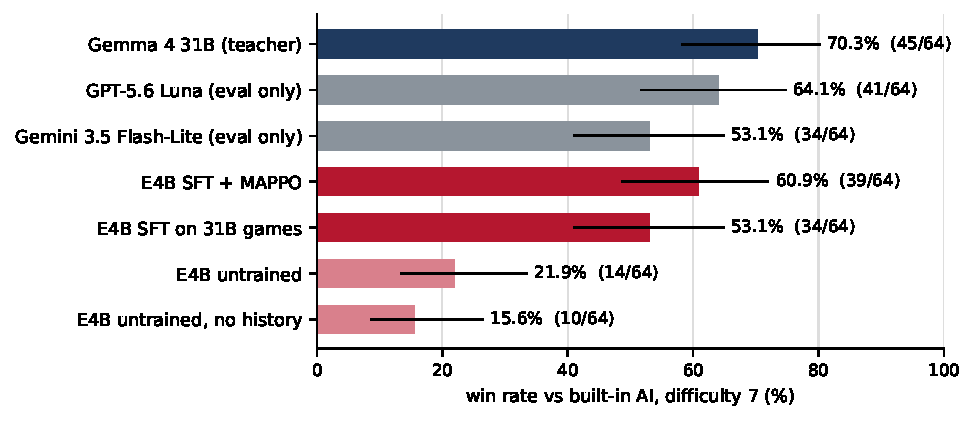
\includegraphics[width=\linewidth]{fig_same_maps.pdf}
\vspace{-6mm}
\caption{Win rate against the built-in AI (difficulty 7) on the same 64 test maps (seeds
200000--200063), with 95\% Wilson intervals. Closed models are evaluation only.}
\label{fig:win}
\end{figure}
\begin{table}[t]
\centering\footnotesize
\caption{Channel and history ablations (development seeds for E4B; 31B: 40 unpaired games per cell).
$b/c$: seeds won only by the first / second condition.}
\label{tab:main}
\begin{tabular}{llrrr}
\toprule
Model & Comparison & win (\%) & $b/c$ & $p$ \\
\midrule
31B & C1 vs C0 & 50 vs 25 & -- & 0.037 \\
31B & C2 vs C0 & 60 vs 25 & -- & 0.003 \\
31B & C2 vs C1 & 60 vs 50 & -- & 0.50 \\
E4B & C1 vs C0 & 18.8 vs 17.2 & 8/7 & 1.0 \\
E4B & C2 vs C0 & 17.2 vs 17.2 & 7/7 & 1.0 \\
E4B & C2 vs C2 no history & 17.2 vs 3.1 & 10/1 & 0.012 \\
\bottomrule
\end{tabular}
\end{table}
\paragraph{Q1: communication helps the large model only.} For Gemma~4 31B, sharing teammates' states
doubles the win rate (25$\to$50\%) and adding free messages reaches 60\%; the C2--C1 step is not
significant. Without any tactic in the prompt, 31B \emph{uses language for focus fire}: 83\% of its
decisions carry a message, 85\% of messages name a target (``focusing e4'', ``finishing e1''), and a
teammate that can hit the named enemy attacks it 70\% of the time vs 45\% by chance (an association:
teammates may pick the same weak enemy independently). The untrained 4B gains nothing from either
channel: its messages are mostly movement chatter (``moving towards action'').
\paragraph{Q2: memory helps the small model, but less than first measured.} On the development seeds,
removing the 5-step history dropped the untrained E4B from 17.2\% to 3.1\% (10 vs 1 maps won only by one
side, $p{=}0.012$). On the 64 test seeds the drop is smaller, 21.9\% to 15.6\% (9 vs 5, $p{=}0.42$):
the direction replicates but the size does not, so the first estimate was inflated by the seed set.
Pooled over both sets (128 maps), history wins 19 maps the no-history model loses and loses 6
($p{=}0.015$).
\paragraph{Q3: learning from 31B works.} SFT on 31B games lifts E4B from 21.9\% to 53.1\% on the test
seeds (25 vs 5 maps won only by one side, $p{<}0.001$; development seeds: 17.2\% to 53.1\%), where the 31B teacher still leads (70.3\%; 17 vs 6 maps, $p{=}0.03$). The trained model also
adopts the teacher's language: messages rise from 23\% to 81\% of decisions and named targets from 40\%
to 88\% of messages (test seeds).
\paragraph{Q4: multi-agent RL on top of SFT (in progress).} Starting from SFT, MAPPO (23 rounds, 368 games) reaches 60.9\% on the test seeds vs 53.1\% for SFT (20 vs 15
maps won only by one side; paired 95\% interval $-9$ to $+27$ points): a gain that is \emph{not yet
established}. Diagnostics show the policy moves little per round (KL to SFT $\approx$0.005--0.01, PPO
clip fraction $<$1\%), consistent with small, slow changes. Gaps between models are mostly on split
starts (SFT 34.5\%, MAPPO 48.3\%, 31B 58.6\%); on grouped starts all are 69--80\%.

\begin{table}[t]
\centering\footnotesize
\caption{Behaviour per model on the same 64 test maps (mean over games). $\dagger$: the paired 95\%
interval (bootstrap over maps) of the change from the column to its left excludes 0
(untrained$\to$SFT and SFT$\to$MAPPO).}
\label{tab:behav}
\setlength{\tabcolsep}{5pt}
\begin{tabular}{lrrrr}
\toprule
 & untrained & SFT & MAPPO & 31B \\
\midrule
win (\%) & 21.9 & 53.1$^\dagger$ & 60.9 & 70.3 \\
win after losing the first unit (\%) & 8 & 23 & 52 & -- \\
invalid orders (\%) & 5.4 & 0.2$^\dagger$ & 0.0$^\dagger$ & 0.6 \\
target switch (\%) & 13.8 & 2.1$^\dagger$ & 2.7 & 2.8 \\
move away, enemy visible (\%) & 28.7 & 6.2$^\dagger$ & 4.4 & 14.6 \\
low-hp retreat (\%) & 42.0 & 25.8$^\dagger$ & 13.7$^\dagger$ & 42.7 \\
stalker kite (\%) & 0.7 & 5.3$^\dagger$ & 1.8$^\dagger$ & 20.5 \\
focus (\%) & 37.7 & 33.7 & 40.6 & 43.7 \\
weakest (\%) & 85.1 & 89.7$^\dagger$ & 90.2 & 92.9 \\
spread in fight & 4.04 & 3.21$^\dagger$ & 2.86 & 3.10 \\
messages naming an enemy (\% of decisions) & 8.9 & 71.5$^\dagger$ & 76.7$^\dagger$ & 73.0 \\
\bottomrule
\end{tabular}
\end{table}
\paragraph{Q5: where do the gains come from?} (Table~\ref{tab:behav}.)
\emph{Untrained$\to$SFT: the squad stops wavering.} SFT does not clearly win the opening (the
untrained model loses a unit first in 61\% of games, SFT in 47\%; the interval includes 0); it wins the
fight that follows (after losing the first unit: 8\%$\to$23\% wins; after killing first:
45\%$\to$83\%; kills per game 3.1$\to$4.2, own losses 4.5$\to$3.7). The untrained model leaves targets
that are still in range (14\% of attacks vs 2\%), walks away from visible enemies (29\% of moves vs
6\%), fights more spread out and issues invalid orders (5\%); it is picked off unit by unit. These
differences are already present in the opening, before any unit dies, so they are a change of play,
not a consequence of winning. SFT also targets the weakest enemy more often and talks like the teacher
(named targets in 72\% of decisions vs 9\%).
\emph{SFT$\to$MAPPO: fewer retreats.} The opening is unchanged (each loses a unit first in 47--48\% of
games); the whole gain is in fights after the first loss (23\%$\to$52\% wins). The significant changes
all point one way: damaged units retreat less (26\%$\to$14\%; when behind 64\%$\to$15\%), stalkers kite
less (5\%$\to$2\%), and all attackers hit one target more often (34\%$\to$41\%, borderline). Retreating
units stop dealing damage; MAPPO learned to keep them in the fight.
\emph{RL does not move the student toward the teacher.} 31B kites (21\%), retreats when damaged (43\%)
and moves away from enemies (15\%) far more than either 4B model. SFT copied 31B's targeting and
messages but not these rarer repositioning moves, which imitation learns poorly; MAPPO moved further
away from them, toward a simpler stay-and-fight strategy. These are correlations from logs; a causal
test (removing teammates' messages at test time) is planned.

\section{Next Steps}
(1) Confirm the RL gain: more MAPPO rounds with larger updates (running) and more test maps (a 10-point gap needs $\sim$300 paired maps for a clear answer).
(2) Causal checks of coordination: drop or shuffle teammates' messages at test time. (3) Cross-game
memory: before a game, agents read a short log of the previous game on the same seed. (4)
Individual-vs-team incentives: give one unit a secret reward and measure free-riding and collusion.

\section{Code}
\url{https://github.com/para2046/cs221-llm-squads}: \texttt{smac\_llm/} (text interface, rewards in
\texttt{game.py}, environment server, SFT in \texttt{train.py}, MAPPO in \texttt{mappo.py}),
\texttt{scripts/} (evaluation and behaviour analysis: \texttt{same\_maps\_table.py},
\texttt{behavior\_shift.py}, \texttt{gain\_analysis.py}).

\section*{AI-Use Disclosure Statement}
We used Claude Code (Anthropic, Claude Opus 5.5) to search and summarise related work, write the
environment adapter, training and analysis code, run the experiments on our cluster, and draft this
report; ChatGPT reviewed a draft and suggested revisions. GPT-5.6 Luna, Gemini~3.5 Flash-Lite and
Inkling-2-Small were used only as evaluated players; no closed-model outputs were used as training
data (the teacher, Gemma~4 31B, is an open-weight model). All design decisions, results and text were
reviewed by the author, who is responsible for the final content. \todo{author to confirm and edit}

\bibliography{references}
\bibliographystyle{iclr2026_conference}

\end{document}
